% \section{Introduction}
% When exposed to naturalistic stimuli (e.g. movie watching), subjects'
% experience is closer to their every-day life than with classical
% psychological experiments.
% %
% This makes naturalistic paradigms an attractive class of
% stimulation protocols for brain imaging.
% %
% While there is a broad interest in understanding how the brain reacts
% in such ecological conditions, the recorded brain activity is
% difficult to analyse.
% %
% Standards methods such as the general linear model \cite{poline2012general} require the experimenter to construct a design matrix that models features of the presented stimuli across time. 
% %
% Such design matrices are notoriously difficult to construct for naturalistic stimuli as one has to rely on manual annotations (see \cite{huth2012continuous}) or deep learning techniques (see e.g. \cite{gucclu2017increasingly}, \cite{eickenberg2017seeing}, \cite{richard2018optimizing} or \cite{gucclu2015deep}) that are hard to use, and provide high-dimensional, cumbersome models of the stimulus.

% \cite{hasson2004intersubject} has shown that brains exposed to the same natural stimuli exhibit synchronous activity.
% %
% The shared response model (SRM) \cite{chen2015reduced} models this behaviour and extracts a common response from different subjects exposed to the same stimuli and subject-specific spatial components.
% %
% The resulting shared response can serve as a design matrix, while the spatial components are naturally seen as weighting factors. 


% SRM has initially been designed to work within regions of interest using few subjects.
% %
% It has been used in \cite{chen2015reduced} to transfer knowledge between subjects allowing precise location of a 15s time segment of fMRI data from a left-out subject using data from other subjects exposed to the same stimuli. 

% A first big step towards more scalability has been made in \cite{anderson2016enabling} reducing fitting time and memory requirements by several orders of magnitude thanks to a smart use of the inversion lemma. 
% %
% After this improvement, studies using larger regions of interest have emerged such as \cite{vodrahalli2018mapping}, which uses SRM to predict text embeddings from fMRI data or \cite{chen2017shared}, which shows that shared memories also come with shared structure in neural activity.
% %
% However, when using full brain data and a large number of subjects and runs, computational costs are still very high. Memory requirements are difficult to meet since all data have to be loaded in memory and since all full brain spatial components of all subjects are updated at each iteration, this leads to a heavy computational burden.


% Fortunately, these high costs can be reduced. Intuitively, since the shared response lives in a reduced space, a compressed representation of the input is good-enough to find a suitable estimate.
% %
% With the use of off-the-shelf atlases and careful memory management we implement this idea and build FastSRM.


% FastSRM is scalable with the number of runs and subjects. Fitting time and memory requirements are reduced considerably, making it possible to fit FastSRM using a laptop in a reasonable amount of time.
% %
% % We also find that the use of atlases limits redundancy and diminishes the noise
% % by smoothing (as seen in \cite{varoquaux:hal-00812911}) yielding slightly better
% % performance than current implementations.
% % %
% FastSRM makes large-scale analysis of movie-watching fMRI fast and easy. We demonstrate its usefulness on CamCAN data where we predict age from movie watching data with a mean absolute error (MAE) of 7.5 years.
% %
% We also show in an encoding experiment that FastSRM's ability to transfer data between subjects is superior to current implementations (\cite{anderson2016enabling}).  

% Our code is freely available at \url{https://github.com/hugorichard/brainiak/tree/fastsrm}.


% There is a long history of using latent factor models for fMRI data analysis.
% %
% ICA was first applied on fMRI data in \cite{mckeown1998analysis} as an alternative to the generalized linear (GLM) model.
% %
% A few years later, \cite{beckmann2004probabilistic} proposed Probabilistic ICA reducing overfitting problems of original ICA by introducing a Gaussian noise model and low rank structure.
% %
% In order to be able to compare patterns across subjects, ICA can be applied on time-wise concatenated data \cite{calhoun2001method}. 
% %
% In 2010, \cite{varoquaux2010group} introduces CanICA that yields more stable group decompositions than previous group ICA methods (\cite{calhoun2001method}, \cite{beckmann2005tensorial} and \cite{smith2004advances}).

% Since then, a number of different factor models have been applied to fMRI data such as non-negative matrix factorization \cite{xie2017decoding} or dictionary learning \cite{varoquaux:inria-00588898}.
% %
% All models enforce constrains on the data that are more or less realistic. \cite{abraham} shows that total variation constrains on spatial components yield accurate and stable decompositions across subjects. However, with high quantities of data, the impact of such regularizations on the result vanishes (see \cite{dohmatob2016learning}) and in this case one should therefore favor efficient algorithms (such as the online dictionary learning implementation of \cite{mensch2016dictionary}).
% %
% In practice, most factor algorithms have been used to derive atlases from rest data. But other applications exist. In \cite{varoquaux2013cohort}, dictionary learning is used to derive an atlas from task data (contrast maps) and ICA is used in \cite{calhoun2004alcohol} and \cite{calhoun2002different} to study respectively the effect of alcohol and speed on driving behavior thanks to a simulated driving protocol.

% SRM has first been introduced in \cite{chen2015reduced}. Like \cite{lashkari2009exploratory}, it learns subject-specific atlases and extracts a shared functional representation from the fMRI data of multiple subjects exposed to the same stimuli.
% %
% It relies on the hypothesis that orthonormality constrains put on spatial components allow for the extraction of more interpretable spatial components from naturalistic-stimulus fMRI data. %
% %
% SRM is not sensitive to the spatial variability of activated area between subjects since the only common features across participants are time courses making up the shared representation.
% %
% It is thus related to template estimation methods such as hyperalignment \cite{guntupalli2016model} or optimal transport \cite{DBLP:conf/ipmi/BazeilleRJT19}.
% %
% Many variants of SRM exists. \cite{chen2016convolutional} uses a convolutional autoencoder to preserve spatial locality, \cite{shvartsman2017matrix} uses matrix normal prior on spatial components and shared response,  \cite{turek2018capturing} adds a subject-specific component and \cite{turek2017semi} gives a semi-supervised version of SRM.
% %
% All of these methods suffer from the efficiency issues already mentioned for standard SRM.
% %
% Note that, unless specified otherwise, whenever we refer to SRM, we refer to the current most efficient implementation of ProbSRM as provided by \cite{anderson2016enabling} which is freely available in the brainiak library \url{https://github.com/brainiak/brainiak}.

% FastSRM needs atlases with a sufficient number of regions to work. Good atlases of various size are available in the literature such as Basc (up to 444 parcels) \cite{bellec2010multi}, Shaeffer (up to 800 parcels) \cite{schaefer2017local} or MODL (up to 1024 parcels) \cite{mensch2018extracting}.
% %
% We show that taking any such atlas yields quantitatively similar results.


In typical fMRI datasets, the number of features $v$ is on the order of $10^5$,
the number of samples $n$ on the order of $10^2-10^3$, the number of views
(subjects) 
$m$ on the order of $10-10^2$ and the desired number of components $p$ on the order
of $10-10^2$.
Therefore, it is quite frequent that fMRI datasets do not hold in memory.
In order to circumvent the problem, most studies apply the shared response model
on regions of interests.

In the following, we present a fast and memory efficient algorithm for
fitting the shared response model on large data allowing practitioners to use
the model on full brain data.

\section{The FastSRM algorithm}
The goal of deterministic srm (respectively probabilistic srm) is to recover mixing matrices $(A_i)_i$ and shared
components $\sbb$ (respectively mixing matrices $(A_i)_i$, noise levels
$(\sigma_i)_i$ and components covariance $\Sigma_s$). 
Let us consider a set of view specific atlases $(U_i)_i \in \RR^{v, r}$ such that
$U_i^{\top}U_i = I_r$.
Data are reduced using $\zb_i = U_i^{\top} \xb_i$ and a SRM algorithm is applied
on $(\zb_i)_i$ yielding parameters $(A_i')_i, \sbb$ (respectively $A_i',
\sigma_i', \Sigma_s$). Then we set $A_i = U_i A'_i$ to recover the mixing matrices.
As we will see in the next section, SRM algorithms may have to be slightly
modified in order to obtain guaranties on the recovered parameters.

The figure~\ref{fig:srm:conceptual} illustrates this process.
\begin{figure}
  \centering
  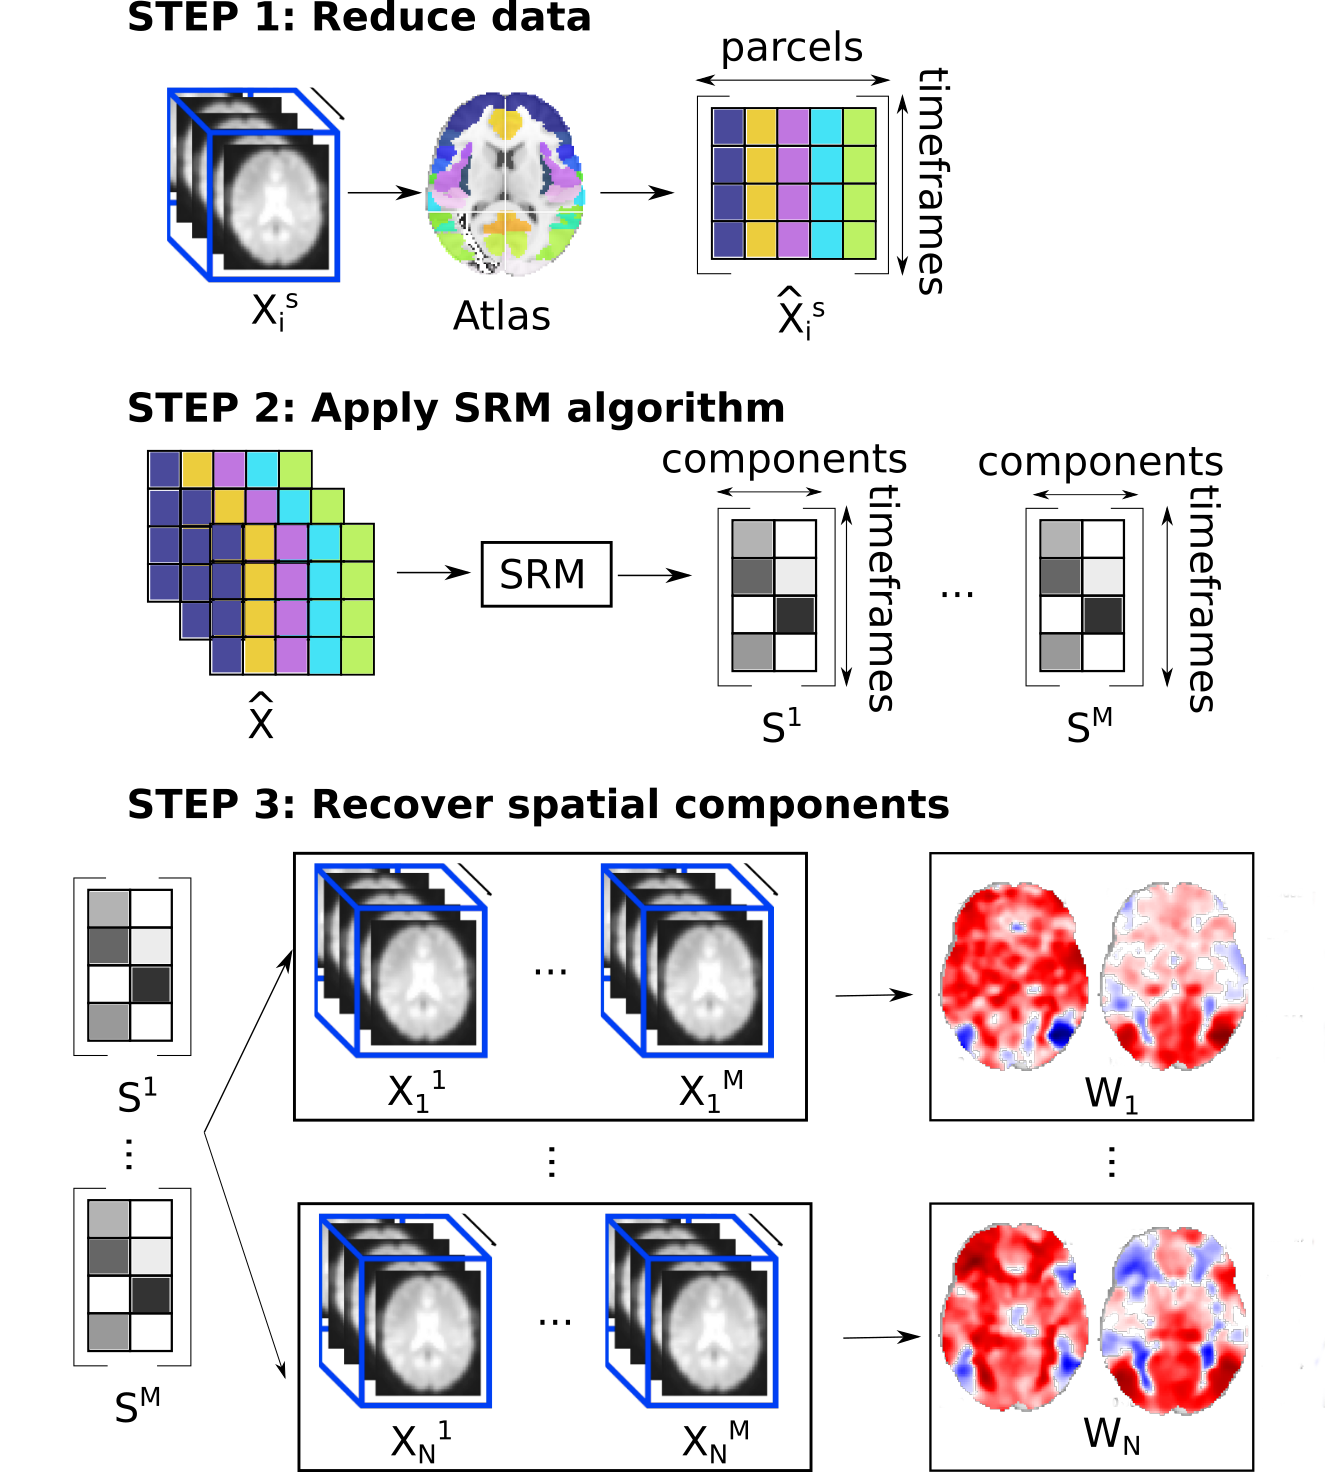
\includegraphics[scale=0.34]{figures/srm/conceptual_figure2.png}
  \caption{\textbf{FastSRM algorithm} In step 1, data are projected onto an atlas (top). In step 2 a deterministic SRM algorithm is applied on reduced data to compute the shared response(middle). In step 3, spatial components are recovered by regression from the shared response (bottom).}
  \label{fig:srm:conceptual}
\end{figure}

From a computational stand point, the optimal dimension reduction provides
a large reduction in memory usage. Indeed as the original data are seen only
once, it is no longer necessary to keep the full dataset in memory (we can load
data $(\xb_i)_i$ one view a time and similarly for the atlases $(U_i)_i$. Therefore the memory consumption is only in $\bigO(vn)$ which is lower than classical SRM algorithms by a factor of $m$. This yields a practical benefit: on most fMRI datasets, one no longer need a large cluster to run the shared response model but only a modern laptop.
Additionally, low memory consumption reduces the
risk of thrashing~\cite{denning1968thrashing}, a phenomenon that causes large
increase in computation time when the memory used is close to the total available
memory in the harware.

After preprocessing, the reduced representation $\zb_i$ is used instead of the
original data $\xb_i$ yielding a time complexity of $\bigO(
\mathrm{T_{preprocessing}} + \mathrm{n_{iter}} mpnr)$.
Let us highlight that in practice, it often happens that an experiment is run
multiple times such as when cross validated results are needed. In these cases,
the pre-processing is performed only once and the apparent complexity becomes
$\bigO(\mathrm{n_{iter}} mpnr)$ which is faster than traditional SRM methods by
a factor of $\frac{v}{r}$.

In general, working with reduced data induces a discrepancy between the result
of the traditional shared response model  and our FastSRM algorithm.
In the next section, we show that there exists an optimal atlas in the sense
that the traditional shared response model and FastSRM will yield the same
results whether it is applied on full data or on reduced data.

\section{Optimal atlases}
Let us consider $\xb_i = U_{\xb_i} \zb_i$ a PCA of $\xb_i$. As the number of
samples $n$ is lower than the number of features $U_{\xb_i} \in \RR^{v, n}$ and
$\zb_i \in \RR^{n}$.  We also have $U_{\xb_i}^{\top}U_{\xb_i} = I$.

As the next property shows, $U_{\xb_i}$ constitutes an optimal atlas when
fitting deterministic SRM.
\begin{prop}[Optimal dimension reduction via PCA for deterministic SRM]
  Let $(A_i)_i, \sbb$ be the solution obtained by deterministic SRM on data
  $\xb_i$ and $(A_i')_i, \sbb'$ the solution obtained by deterministic SRM on
  data $\zb_i = U_{\xb_i}^{\top} \xb_i$. Then $A_i = U_{\xb_i}A_i'$ and $\sbb = \sbb'$. 
\label{prop:optimaldetsrm}
\end{prop}
\begin{proof}
Updates of the mixing matrices $A_i$ in deterministic SRM
equation~\eqref{eq:detsrm:Aiupdate} can be written:
\begin{align}
  A_i &\leftarrow \Pcal(\xb_i \sbb^T) \\
      &\leftarrow U_{\xb_i}\Pcal(\zb_i \sbb^T)
\end{align}

Therefore we can look for $A_i$ as $A_i = U_{\xb_i} \tilde{A_i}$. $\tilde{A_i}$ is
orthogonal. Indeed
\begin{align}
  &A_i^{\top} A_i = I_p \\
  & \implies \tilde{A_i}^{\top}U_{\xb_i}^{\top} U_{\xb_i} \tilde{A_i} = I_p \\
  & \implies \tilde{A_i}^{\top} \tilde{A_i} = I_p
\end{align}

Then, we use the fact that
\begin{align}
  \|\xb_i - A_i \sbb \|^2 = \| U_{\xb_i}\zb_i - U_{\xb_i}\tilde{A_i} \sbb\|^2 = \| \zb_i - \tilde{A_i} \sbb \|^2
  \label{eq:equality:xy}
\end{align}
Therefore, there the solution of deterministic SRM on data $(\zb_i)_i$ and
$(\xb_i)_i$ are linked by the change of parameters $A_i = U_{\xb_i}A_i'$ and
$\sbb = \sbb'$ where $A_i' = \tilde{A_i}$. This concludes the proof.
\end{proof}
In the case of probabilistic SRM we can obtain very similar results however the
algorithm applied on reduced data need to be slightly modified.
We call probSRM($\nu$) the probabilistic SRM algorithm modified such that
updates
\begin{align}
\sigma_i^2 \leftarrow \frac1{v} (\| \xb_i - A_i \EE[\sbb|\xb]\|^2 + \| \diag(\VV[\sbb | \xb]) \|^2)
\end{align}
are replaced by updates
\begin{align}
  \sigma_i^2 \leftarrow \frac1{\nu} (\| \xb_i - A_i \EE[\sbb|\xb]\|^2 + \| \diag(\VV[\sbb | \xb]) \|^2)
\end{align}

We have the following result:
\begin{prop}[Optimal dimension reduction via PCA for probabilistic SRM]
  Let $(A_i)_i, \sigma_i, \Sigma_s$ be the solution obtained by probabilistic SRM on data
  $\xb_i$ and $(A_i')_i, \sigma_i', \Sigma_s'$ the solution obtained by ProbSRM($v$) on
  data $\zb_i = U_{\xb_i}^{\top} \xb_i$.Then $A_i = U_{\xb_i}A_i'$, $\sigma_i =
  \sigma_i'$ and $\Sigma_s = \Sigma_s'$. 
  \label{prop:optimalprobsrm}
\end{prop}
\begin{proof}
  A similar reasoning can be done with probabilistic SRM starting from
  equation~\eqref{eq:srm:Aiupdate} gives:
  \begin{align}
    A_i &\leftarrow U_{\xb_i}\Pcal(\zb_i \EE[\sbb| \xb_i]^T)
  \end{align}
  so we can look for $A_i$ as $A_i = U_{\xb_i} \tilde{A_i}$ and, as in the
  deterministic case, $\tilde{A_i}$ is orthogonal.
  Therefore equality~\eqref{eq:equality:xy} holds.
  
  Then we consider the negative log-likelihood of probabilistic srm:
  \begin{align}
    \loss &= \sum_i \frac12 v\log(\sigma_i^2) + \frac12 \log(|\Sigma_s|) + \int_{\sbb} \sum_i \frac1{2 \sigma_i^{2}}\|\xb_i - A_i \sbb \|^2 + \frac12 \langle \sbb , \Sigma_s^{-1} \sbb \rangle  d\sbb \\
    &= \sum_i \frac12 v \log(\sigma_i^2) + \frac12 \log(|\Sigma_s|) + \int_{\sbb} \sum_i \frac1{2 \sigma_i^{2}}\|\zb_i - \tilde{A_i} \sbb \|^2 + \frac12 \langle \sbb , \Sigma_s^{-1} \sbb \rangle  d\sbb
  \end{align}
  where we use equality~\eqref{eq:equality:xy}.
  Optimizing the log-likelihood via expectation maximization yields the exact
  same updates as probabilistic srm on data $\zb_i$
  except that updates
  \begin{align}
    \sigma_i^2 \leftarrow \frac1{t} (\| \zb_i - \tilde{A_i} \EE[\sbb|\zb]\|^2 + \| \diag(\VV[\sbb | \zb]) \|^2)
  \end{align}
  are replaced by updates
  \begin{align}
    \sigma_i^2 \leftarrow \frac1{v} (\| \zb_i - \tilde{A_i} \EE[\sbb|\zb]\|^2 + \| \diag(\VV[\sbb | \zb]) \|^2)
  \end{align}

  The trajectory of both algorithms are linked by $A_i = U_{\xb_i}A_i'$ where
  $A_i' = \tilde{A_i}$, $\sigma_i' =
  \sigma_i$ and $\Sigma_s'  = \Sigma_s$.

  This concludes the proof.
\end{proof}

The properties~\ref{prop:optimaldetsrm} and~\ref{prop:optimalprobsrm} show that
no information is lost by replacing $\xb_i \in \RR^v$ by its reduced representation $\zb \in \RR^n$.
A key property of the optimal atlas $U_{\xb_i}$ is that it is valid whether or
not the model for deterministic (respectively probabilistic) SRM holds.

A complexity analysis  shows that finding the optimal atlas becomes the limiting step of the pipeline. The time complexity becomes $\bigO(mvn^2)$ which is faster than classical SRM implementations only if $n < n_{iter} p$. However, in popular
linear algebra pipeline such as scipy~\cite{2020SciPy-NMeth}, the code
performing singular value decomposition is highly optimized therefore the
constant in front of the $\bigO$ is low. Lastly, if more memory is available, finding the optimal atlas can be done in parallel for each view, trading memory for time.

In the next section, we investigate approaches to reduce the preprocessing time.

\section{Efficient approximation of optimal atlases}
As we have seen in the previous section, if $U_i = U_{\xb_i}$ where $\xb_i =
U_{\xb_i} \zb_i$ is a PCA of $\xb_i$, then $U_i$ is an optimal atlas.
A natural follow-up is to look for atlases that are close to optimal in the
sense that the inertia $\| (I - U_i U_i^{\top}) \xb_i \|$ is low but are fast to
compute and such that projecting data on the atlas is a cheap operation.

Deterministic atlases are interesting as they allow for fast data projection
(computing $U_i \xb_i$ only costs $\bigO(v)$). Furthermore, they are thought to
be more suited to fMRI data as they filter noise via smoothing (this argument is
detailed in~\cite{hoyos2018recursive}).

A first approach is to use existing deterministic atlases for fMRI data such as 
~\cite{schaefer2017local} or~\cite{bellec2010multi}. As theses atlases
attempt to reduce the dimension of fMRI signals without losing too much signal,
there is hope for the inertia to be small.
The clustering approach
of~\cite{hoyos2018recursive} is also appealing as it is optimized to give low
inertia while the cost of finding the deterministic atlas is low (computing $U_i$ only costs
$\bigO(vn)$). As the number $r$ of regions increases, the inertia decreases
and the approximation becomes better and better. 
Lastly, an other good approximation of the optimal atlas is given by performing a PCA with a
number of components $r < n$.

With these approaches, and provided $r$ is low enough, the pre-processing time can be neglected and therefore we
get the time complexity $\bigO(\mathrm{n_{iter}} mpn^2)$ which is faster than
standard implementations by a factor $\frac{v}{n}$.
